%!TEX root=masterproef.tex

\chapter{Hardwareplatform}
\label{hardware-platform}

Voor het hardwareplatform werd gekozen om niet te vertrekken van een bestaand
platform, zoals Arduino \citep{url:arduino} of Atmel RZRaven
\citep{manual:rzraven}. Wel werd geopteerd om te vertrekken van elementaire
componenten: een Atmel ATMEGA1284p \mcu \citep{datasheet:atmega1284p}, een Digi
XBee-module \citep{manual:xbee} en een MAX232 seri\"ele driver-module
\citep{datasheet:max232}.

De beweegreden vindt zijn oorsprong in het aspect betreffende
\emph{standaardisatie} uit de probleemdefinitie (zie sectie
\ref{section:problem-definition}). De keuze van elementaire bouwstenen
reduceert het hardwareplatform tot zijn essentie. De implementatie van de
oplossing kan immers geen gebruik maken van specifieke voorzieningen en dient
alle functionaliteit zelf te voorzien.

Hierdoor is een prototype, gebaseerd op dit platform, representatief voor het
eenvoudigste platform en zal elke toevoeging in de vorm van een uitgebreider
hardwareplatform, slechts meer stabiliteit en mogelijkheden bieden, die de
ontwikkeling louter positief kunnen be\"invloeden.

\section{Minimale noden en voorzieningen}

We overlopen kort de noden en hoe deze voorzien zijn in het platform:

\begin{description}

  \item[Rekenkracht en geheugen] De Atmel ATMEGA1284p is een veelgebruikte
  \mcu. We vinden hem o.a. terug in de populaire Atmel RZRaven ontwikkelingskit
  en op veelgebruikte versies van het Arduino-platform. Hij beschikt over 128KB
  programmeerbaar geheugen en 16KB werkgeheugen. Daarnaast beschikt deze \mcu
  over twee USART seri\"ele poorten.
  
  \item[Draadloos netwerk] \'E\'en van deze poorten kan gebruikt worden voor de
  aansturing van de Digi XBee-module. Deze module biedt met een eenvoudige
  seri\"ele interface toegang tot een ZigBee-netwerk. De eenvoudige interface
  laat toe om bytes te versturen en te ontvangen en implementeert een minimale
  ondersteuning voor het ZigBee-protocol.
  
  \item[Communicatie] Om in parallel met het draadloze netwerk te kunnen
  communiceren met een computer en zo bijkomende informatie te kunnen weergeven
  betreffende de werking van de implementatie, is een MAX232 seri\"ele
  driver-module voorzien. Deze laat toe om via een seri\"ele verbinding en een
  terminal een byte-geori\"enteerde communicatie te realiseren.
  
  \item[Indicatoren] Enkele LEDs (\emph{Light Emitting Diode}) geven
  elementaire feedback over de werking van het ontwerp. Een rode LED geeft aan
  dat het platform onder spanning staat en twee LEDs, oranje en geel, geven
  respectievelijk de beschikbaarheid van het draadloze netwerk en de
  operationele status van de XBee-module aan.
  
\end{description}

\section{Ontwerp}

Figuur \ref{fig:hardware-platform-schematic} toont het schema van het platform.

\begin{figure}[ht]
  \centering
  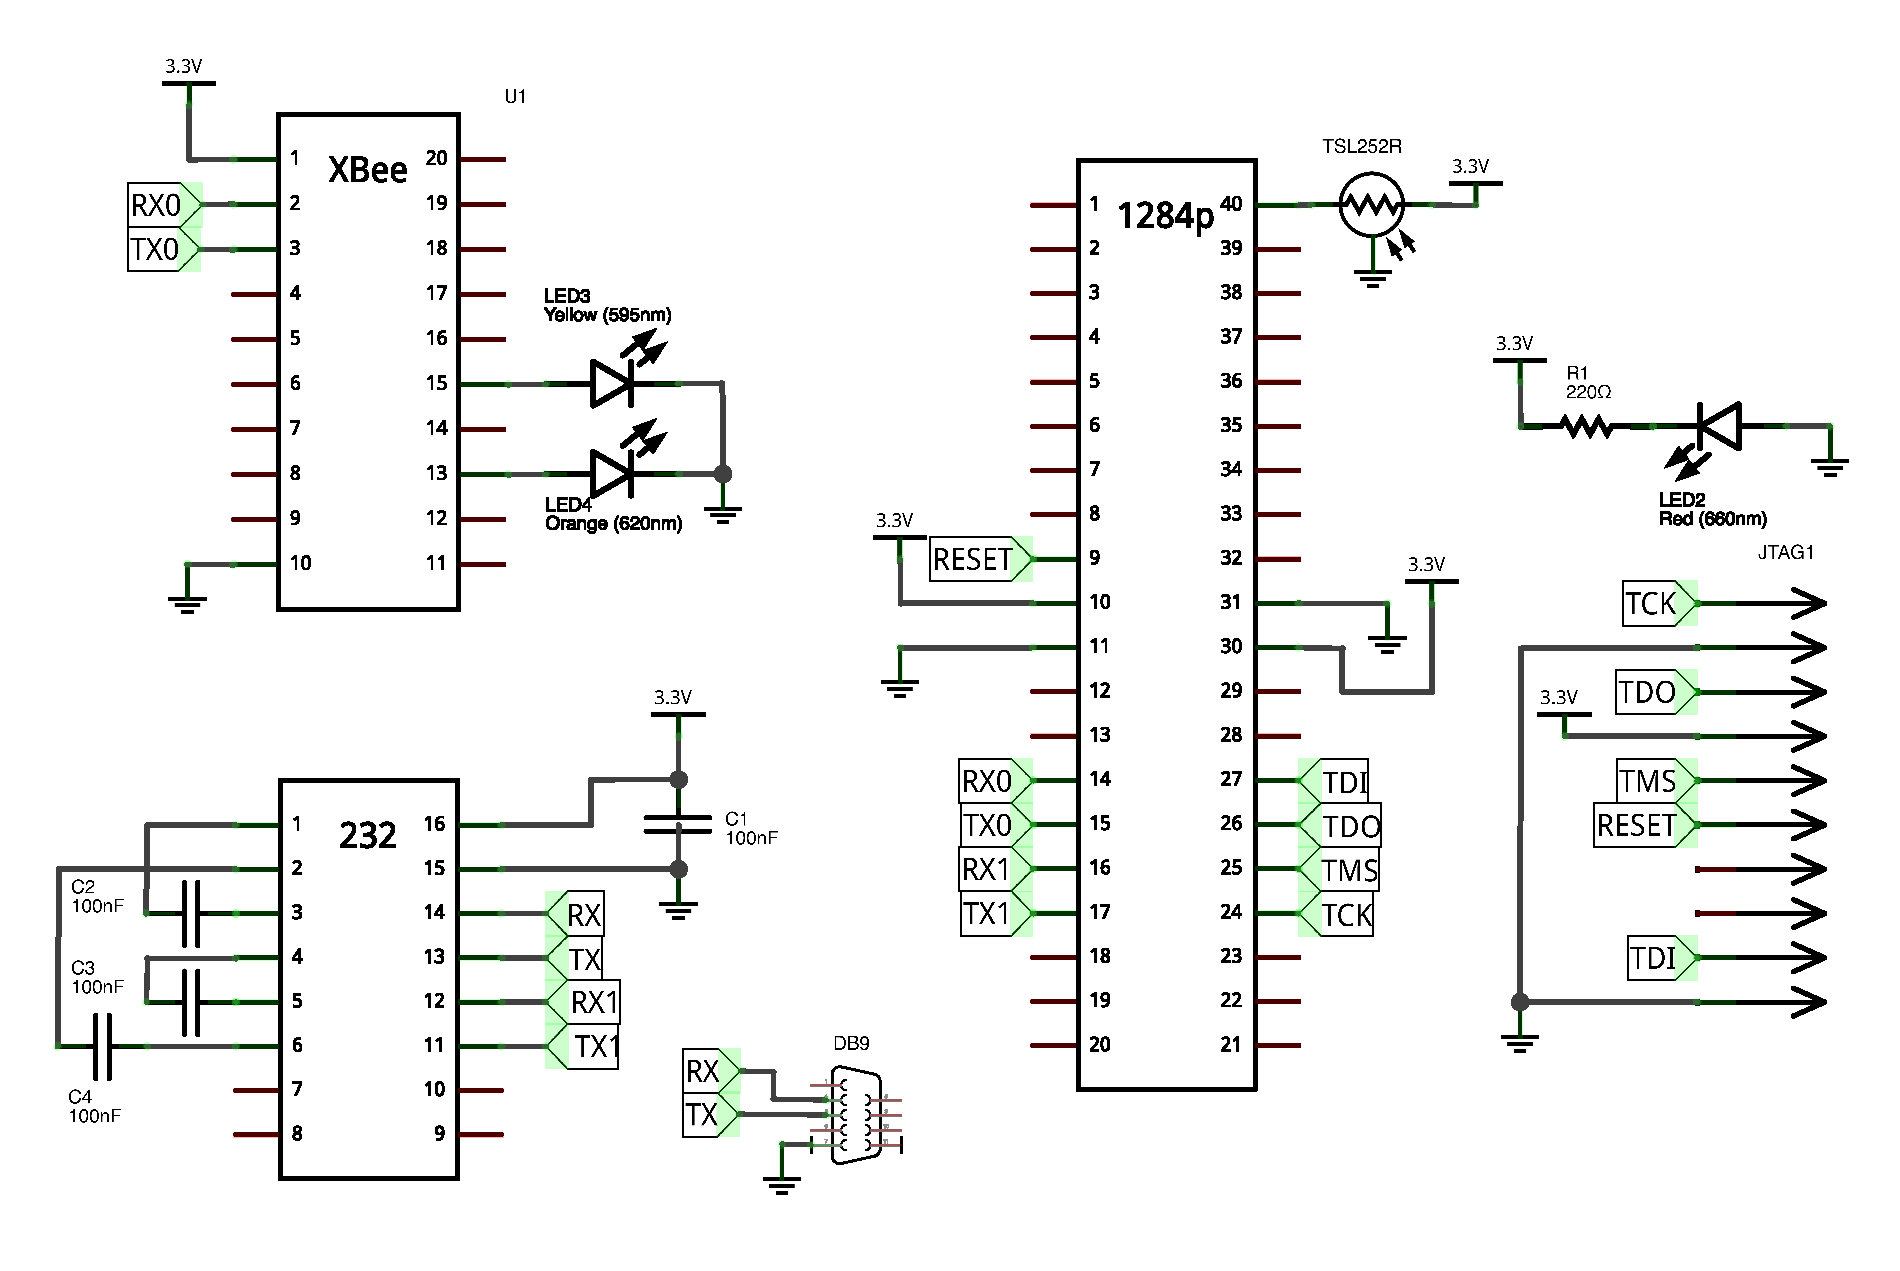
\includegraphics[width=\linewidth]{resources/hardware-platform-schematic.pdf}
  \caption{Schema van hardwareplatform}
  \label{fig:hardware-platform-schematic}
\end{figure}

Op het schema herkennen we de verschillende componenten: centraal de
ATMEGA1284p, met rechts bovenaan de lichtsensor (TSL252R). Rechts daarvan is de
rode LED indicator en de JTAG aansluiting weergegeven. Links bovenaan vinden we
de XBee-module met twee indicatoren en twee seri\"ele verbindingen voor het
versturen en ontvangen van bytes. Tot slot is er links onderaan de
MAX232-module, met verbindingen naar de tweede USART en een DB9-connector.
